\chapter{Introduction}

\section{Background and Motivation}

\subsection{ReVolt}
ReVolt was born out of the increasing need to decongest roads of land-based transport vehicles. Currently, the maritime solution to transport of goods short distances is more expensive and more dangerous than land-based transport. In order to solve these problems, ReVolt is aimed to be an emission free, unmanned vessel. If full autonomy is achieved and no personnel is required on board, the risk for life-threatening situations is nearly completely eliminated. This also vastly reduces the labor cost in the operation of the vehicle. By being emission free, the costs associated with maintenance are greatly reduced in comparison to traditional diesel engines \cite{dnvglRevolt}.

DNV GL bought the ReVolt model boat from Stadt Towing Tank, as a manually controlled vehicle. The model is a 1:20 scale model of ReVolt (which will be referred to as the ReVolt model). DNV GL has since partnered with NTNU to develop the ReVolt model as a test platform for the autonomous functions of the vehicle. One important step in the automatization of the model ReVolt was the development of the Dynamic Position System, which was done in the Spring of 2017 \cite{alfheimMuggerudThesis}.

Over the summer, further work was done improving the boat by three summer students. The main focus areas for the summer were restructuring the flow of data in ReVolt, adding an emergency stop, beginning development of a visualization application in Unity, etc., etc., etc.

\todo[inline]{Get a draft of previous paragraph going with ALbert and Vegard}

\subsection{Digital Twin}
The growth of autonomy is inevitable, however, still quite new. It is developing rapidly in the aviation, automotive and maritime industries. We have cars, planes and boats that are capable of driving themselves, but we are not confident enough in these systems to completely switch to unmanned systems.

In order to help analyze and refine the many facets of an unmanned, autonomous vehicle, we turn to the data we have. As the world grows ever more connected and technology is able to collect and store larger and larger amounts of data, a possibility opens to produce incredibly detailed vehicle simulations. These simulations are not based entirely on first principle physics models, but rather take massive amounts of data collected from the vehicles' sensors and combine them with the existing models to describe a much clearer picture of the system. These simulations are meant to be connected to the physical vehicle all the time and mimic, in real-time, every aspect of the physical vehicle. They are therefore dubbed 'digital twins.' Furthermore, these digital twins live in simulated, virtual worlds, which are also meant to emulate real world conditions for the vehicle(s).

For ships, this type of simulation can lead to advancements in safety and operational efficiency, while achieving the goals of ReVolt by reducing operational cost and environmental impact. 

In the early phases of the project, testing of the control systems can be aided by the data retrieved from the ReVolt test model. By simulation in the digital world, testing can be executed both quicker and with more accurate models. This testing can create a safer vehicle, as the 'digital twin' has completed safety critical tests or high risk maneuvers several thousand times in varying conditions before these same tests and maneuvers are attempted on the physical vehicle.

During the operational phase of ReVolt, historical data of the vehicle can be accrued. This data can be used to make predictions about the lifespan of different components under certain conditions, and possible points of failure in order to save money and increase efficiency. Furthermore, examination of similar data can lead to reduced environmental effects.

When the vehicle is decommissioned, I like to believe that the digital twin lives on in a heaven of sorts for decommissioned vehicles (source: Black Mirror, Season 3 Episode 4, San Junipero).

\begin{figure}[H]
\centering
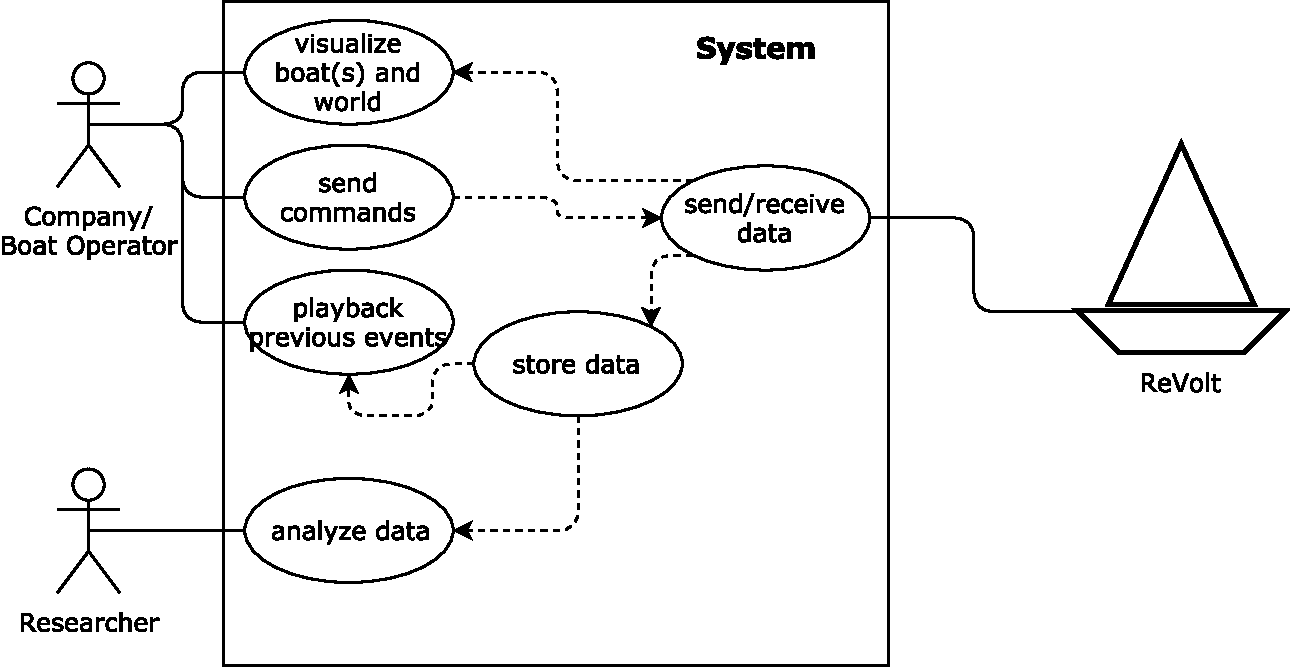
\includegraphics[scale=.6]{Images/Use_Case_Diagram.pdf}
\caption{Potential use cases for ReVolt Digital Twin system}
\label{fig:UseCaseDiagram}
\end{figure}
\todo[inline]{add simulation and obstacle adding}

\section{State of the Art}
While the focus of this report is ships, specifically DNV GL's ReVolt test platform, the idea of a digital twin living in a virtual world is not confined to the maritime industry. 

\todo{Talk about Google and Tesla}

add lit review here

\section{Scope}
In order to develop methods of analyzing and using the data generated from the ship, a system needs to be set up to collect, store, process and visualize the data. The building of this system, a digital twin living in a virtual world, is the focus of this project. In order to build this tool, the model ReVolt needs to be developed into an IoT (Internet of Things) device. The tool will then consist of an IoT Hub and a web application. The IoT Hub runs in the cloud and is used for data collection, storage, processing and analytics. While the web application is used for visualization of ReVolt and the world.

Analysis of the twin data, and developments in methods of using this tool is not within the scope of this project, but rather will be analyzed next semester.

\section{Project Description}
\begin{figure}[H]
\centering
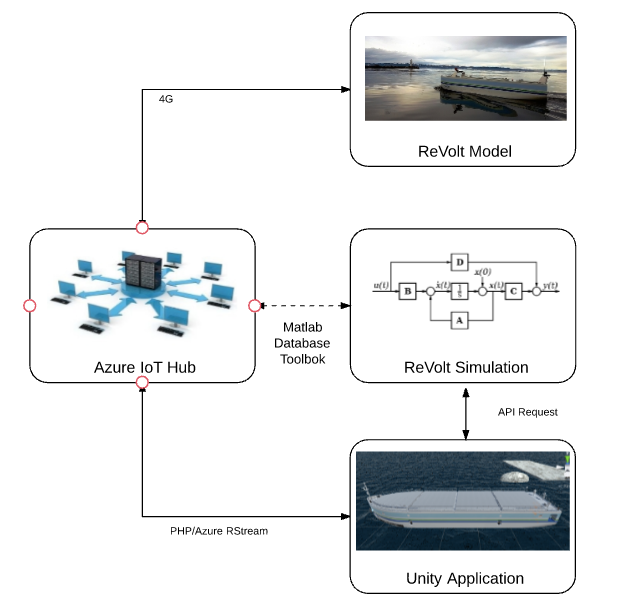
\includegraphics[scale=1.0]{Images/ProjectDescription.png}
\caption{Overview of the main parts of the project and the connections between them.}
\label{fig:ProjectDescription}
\end{figure}

\Cref{fig:ProjectDescription} shows the 4 main segments of the project, as well as the connections between them. 
\begin{description}
 \item[1.] Unity Application
 
 This application mimics the physical system from data that it receives, thereby serving as a visualization of ReVolt. In addition, virtual object locations can be transmitted from the application to the model ReVolt.
 \item[2.] Azure IoT Hub
 
 The Azure IoT Hub is a cloud service provider, that includes data storage, process, and analysis functionality. Data, both archived or real-time, can be sent to the virtual Unity application in order to drive the virtual boat and enhance the world around the virtual boat (e.g. obstacles and waves).
 \item[3.] Simulator Connection
 
 In the absence of the physical boat, or when simulator testing is desired, the model is able to connect to the ReVolt simulator, and collect data from the simulator in order to drive the virtual ReVolt and enhance the world around the virtual boat (e.g. obstacles and waves).
 \item[4.] Model ReVolt
 
 The model ReVolt will send and receive important telemetry data to and from the Azure IoT Hub and the Unity Application.
\end{description}







\section{Requirements}
Each of the described sections has a set of testable requirements to which the success of the project will be evaluated. These requirements to the project are enumerated in \Cref{tab:unityReqs,tab:AzureReqs,tab:SimReqs,tab:BoatReqs}. A set of tests is created which must be passed in order to ensure the completion of all requirements. An over view of which tests cover which requirements is found in \Cref{tab:testOverview}.

\begin{table} [h!]
\caption{Unity Application Requirements}\label{tab:unityReqs}
\centering
\begin{tabulary}{ \linewidth }{|C|L|L|}
    \hline
    \multicolumn{3}{|c|}{\textbf{1. Unity Application}} \\
     \hline
    \textbf{Req. Code} & \multicolumn{1}{|c|}{\textbf{Requirement}} & \multicolumn{1}{|c|}{\textbf{Test}} \\ 
    \hline
    1.1 & The application shall include a virtual ReVolt ship, accurate to the design of the real world ReVolt & Unity Acceptance Test \\ 
    \hline
    1.2 & The application shall include an ocean which shall be in sync with wave force calculations & Unity Acceptance Test \\ 
    \hline
    1.3 & The application shall include obstacles that can be placed by the user & Unity Acceptance Test \\ 
    \hline
    1.4 & The application shall run as a web app & Unity Acceptance Test \\ 
    \hline
    1.5 & The application shall indicate when the virtual boat collides with an obstacle & Unity Acceptance Test \\ 
    \hline
    1.6 & The application shall have an option to update based on data received from the Simulator & Unity-Simulator Connection Test \\ 
    \hline
    1.7 & The application shall have an option to update based on data received from the Azure IoT Hub & Unity-Azure Connection Test \\ \hline
    1.8 & The application shall have an option to send control commands to the Azure IoT Hub &  Unity-Azure Connection Test \\ \hline
\end{tabulary}
\end{table}


\begin{table} [h!]
\caption{Azure IoT Hub Requirements}\label{tab:AzureReqs}
\centering
\begin{tabulary}{ \linewidth }{|C|L|L|}
    \hline
    \multicolumn{3}{|c|}{\textbf{2. Azure IoT Hub}} \\
     \hline
    \textbf{Req. Code} & \multicolumn{1}{|c|}{\textbf{Requirement}} & \multicolumn{1}{|c|}{\textbf{Test}} \\ 
    \hline
    2.1 & The IoT Hub shall be able to collect and store all data sent from the physical ReVolt & ReVolt-Azure Connection Test \\ 
    \hline
    2.2 & The IoT Hub shall be able to send control signals to the physical ReVolt & ReVolt-Azure Connection Test \\ 
    \hline
    2.3 & The IoT Hub shall be able to send data to the Unity model & Unity-Azure Connection Test \\ 
    \hline
    2.4 & The IoT Hub shall be able to receive control signals from the Unity Model, process and save them & Unity-Azure Connection Test \\ 
    \hline
    2.5 & The IoT Hub shall be able to process data as it is received & Azure Acceptance Test \\
    \hline
    2.6 & Incoming data shall be processed at a minimum rate of 20 Hz & Data Rate Test \\ 
    \hline
    2.7 & Data shall be sent onward to the Unity model at a minimum rate of 20 Hz & Data Rate Test \\ 
    \hline
    
\end{tabulary}
\end{table}

\begin{table} [h!]
\caption{Simulator Connection Requirements}\label{tab:SimReqs}
\centering
\begin{tabulary}{ \linewidth }{|C|L|L|}
    \hline
    \multicolumn{3}{|c|}{\textbf{3. Simulator Connection}} \\
     \hline
    \textbf{Req. Code} & \multicolumn{1}{|c|}{\textbf{Requirement}} & \multicolumn{1}{|c|}{\textbf{Test}} \\ 
    \hline
    3.1 & The simulator shall be able to send data to the Unity model & Unity-Simulator Connection Test \\ 
    \hline
\end{tabulary}
\end{table}

\begin{table} [h!]
\caption{ReVolt Model Requirements}\label{tab:BoatReqs}
\centering
\begin{tabulary}{ \linewidth }{|C|L|L|}
    \hline
    \multicolumn{3}{|c|}{\textbf{4. ReVolt Model}} \\
     \hline
    \textbf{Req. Code} & \multicolumn{1}{|c|}{\textbf{Requirement}} & \multicolumn{1}{|c|}{\textbf{Test}} \\ 
    \hline
    4.1 & The ReVolt model shall be able to send data and receive commands to and from the Azure IoT Hub & ReVolt-Azure Connection Test \\
    \hline
    4.2 & The boat shall be able to send data at a minimum rate of 20 Hz & Data Rate Test \\
    \hline
\end{tabulary}
\end{table}

\begin{table} [h!]
\caption{Test Overview}\label{tab:testOverview}
\centering
\begin{tabulary}{ \linewidth }{|L|L|}
    \hline
    \textbf{Test} & \multicolumn{1}{|c|}{\textbf{Requirement Fulfilled}}  \\ 
    \hline
    Unity Acceptance Test & 1.1-1.5 \\
    \hline
    Unity-Simulator Connection Test & 1.6, 3.1 \\
    \hline
    Unity-Azure Connection Test & 1.7-1.8, 2.3-2.4 \\
    \hline
    ReVolt-Azure Connection Test & 2.1-2.2, 4.1 \\
    \hline
    Data Rate Test & 2.6-2.7, 4.2 \\
    \hline
\end{tabulary}
\end{table}